\documentclass[11pt, a4paper]{article}
%\usepackage{proj1}
\usepackage{natbib}
\usepackage{fancyhdr}  
\usepackage{subcaption}
\usepackage{caption}
\usepackage{graphicx}
\usepackage{numprint}
\usepackage{multirow}
\linespread{1.25} 
\setlength{\parindent}{0cm}
\graphicspath{{Images/}}
\usepackage{hyperref}
\usepackage{amsmath}
\usepackage{amsfonts}
\usepackage{amssymb}
\usepackage{amsthm}
\usepackage{mathtools}
\usepackage{commath}
\usepackage{bbm}

%\usepackage[sc,osf]{mathpazo}
\usepackage{subcaption}
\usepackage[a4paper, top=1in, left=1.0in, right=1.0in, bottom=1in, includehead, includefoot]{geometry} %Usually have top as 1in

\usepackage{listings}
\usepackage{color} %red, green, blue, yellow, cyan, magenta, black, white
\definecolor{mygreen}{RGB}{28,172,0} % color values Red, Green, Blue
\definecolor{mylilas}{RGB}{170,55,241}


\hypersetup{colorlinks,linkcolor={black},citecolor={blue},urlcolor={black}}
\usepackage{color}
\urlstyle{same}


\theoremstyle{definition}
\newtheorem{definition}{Definition}[section]

\newcommand{\adja}{q_a}
\newcommand{\adjb}{q_b}
\newcommand{\adjaB}{q_{a,\partial \Omega}}
\newcommand{\adjbB}{q_{b,\partial \Omega}}
\newcommand{\adjB}{q_{\partial \Omega}}
\newcommand{\Adja}{\mathbf{p}}
\newcommand{\Adjb}{q}
\newcommand{\adj}{q}
\newcommand{\Adjc}{{q}_{\partial \Omega}}
\newcommand{\ra}{\rho_a}
\newcommand{\rb}{\rho_b}
\newcommand{\w}{\mathbf{w}}
\newcommand{\f}{\mathbf{f}}
\newcommand{\ve}{\mathbf{v}}
\newcommand{\n}{\mathbf{n}}
\newcommand{\h}{\mathbf{h}}
\newcommand{\K}{\mathbf{K}}
\newcommand{\hr}{\widehat \rho}
\newcommand{\jf}{\mathbf j}

\DeclareMathOperator{\sgn}{sgn}
\DeclareMathOperator{\Grad}{Grad}
\DeclareMathOperator{\Div}{Div}
\DeclareMathOperator{\Lap}{Lap}

%	\begin{figure}[h]
%		\centering
%		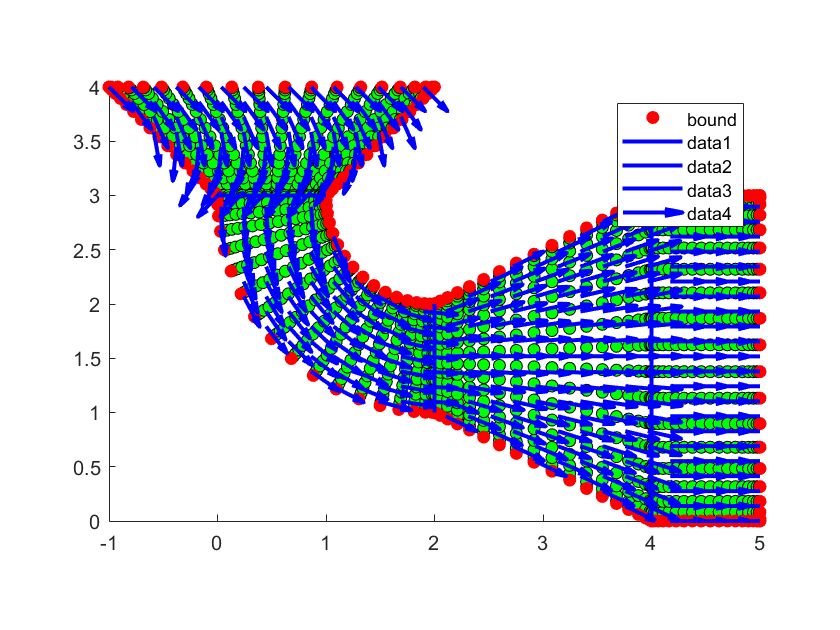
\includegraphics[scale=0.35]{F1.png}
%		\caption{Forward $\rho$ for $a = 0.01$} 
%		\label{F1}
%	\end{figure}

\begin{document}
\section*{Validation Tests}


\section{Testing Differentiation, Interpolation, Convolution and Integration}
TablesDiffIntetc() in Matlab
	\begin{figure}[h]
	\centering
	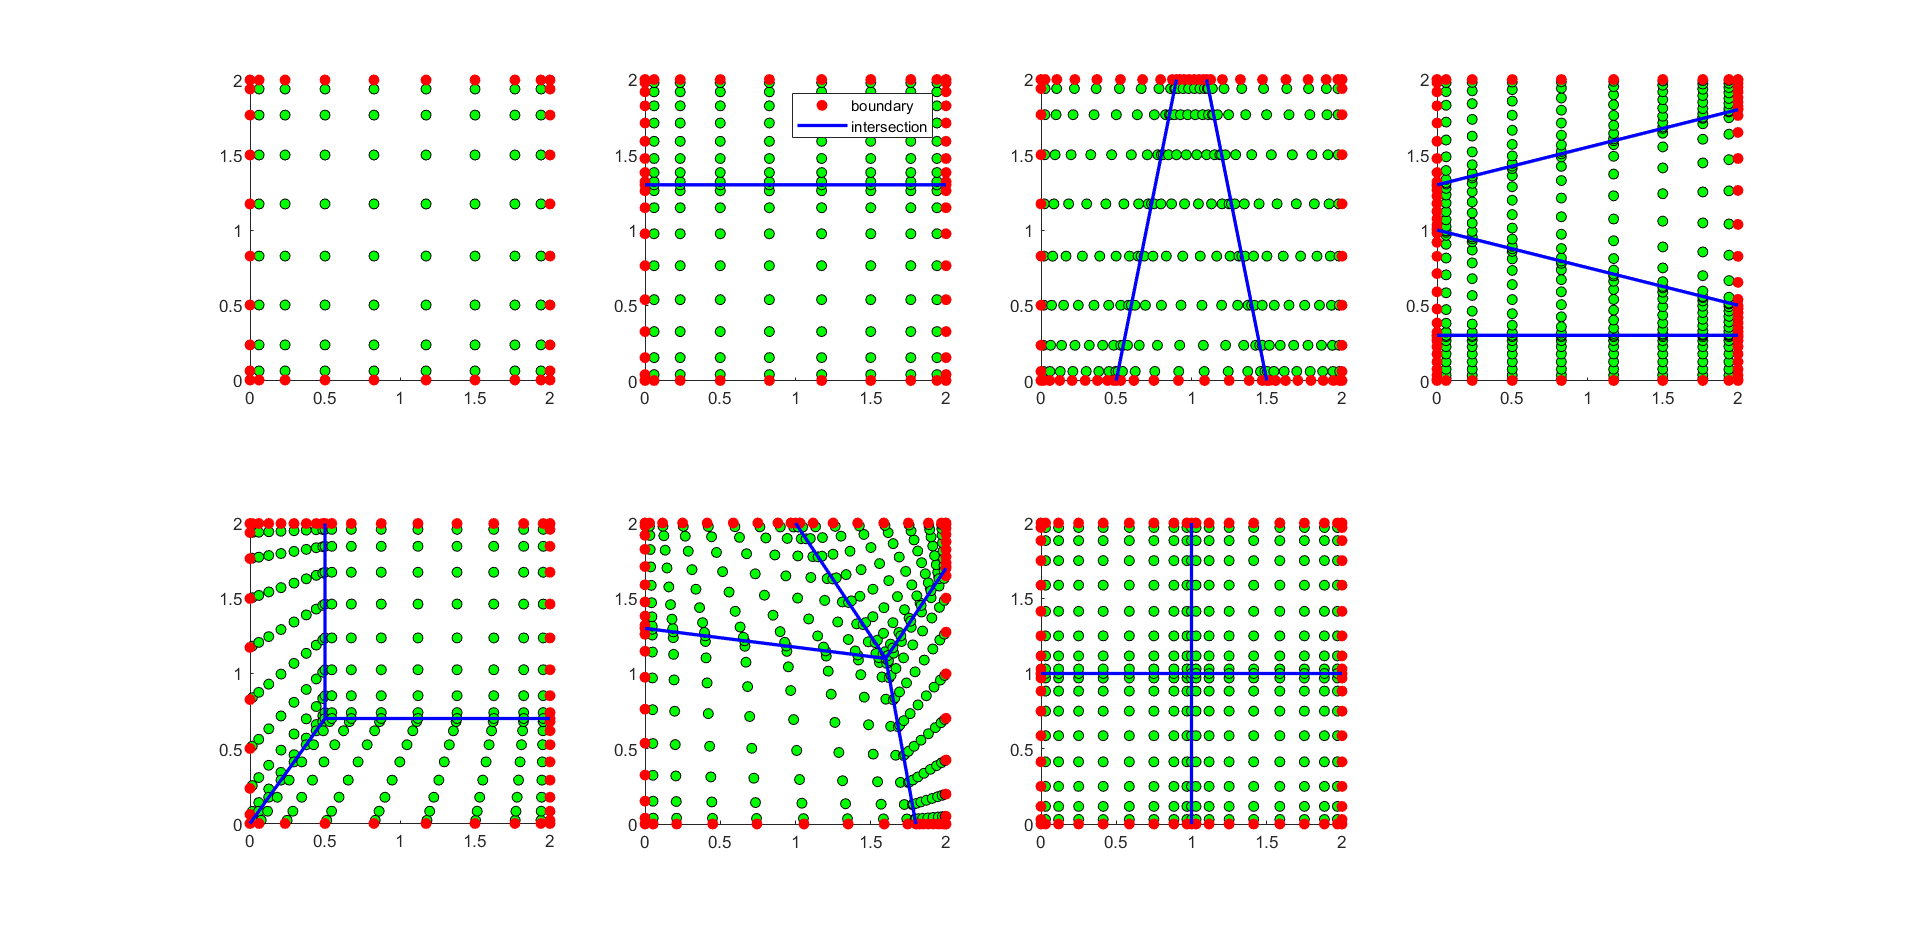
\includegraphics[scale=0.35]{BoxSections.png}
	\caption{Different discretizations of the box (a - g).} 
	\label{F2}
\end{figure}
\begin{figure}[h]
	\centering
	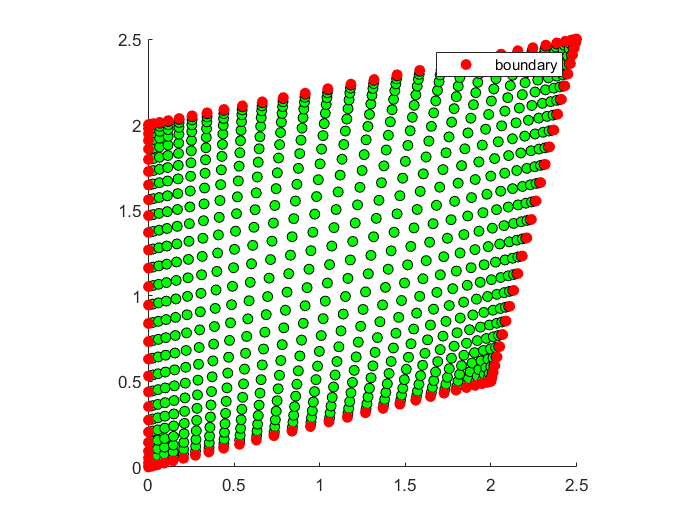
\includegraphics[scale=0.35]{quad.png}
	\caption{Quadrilateral domain (q).} 
	\label{F3a}
\end{figure}
\begin{figure}[h]
	\centering
	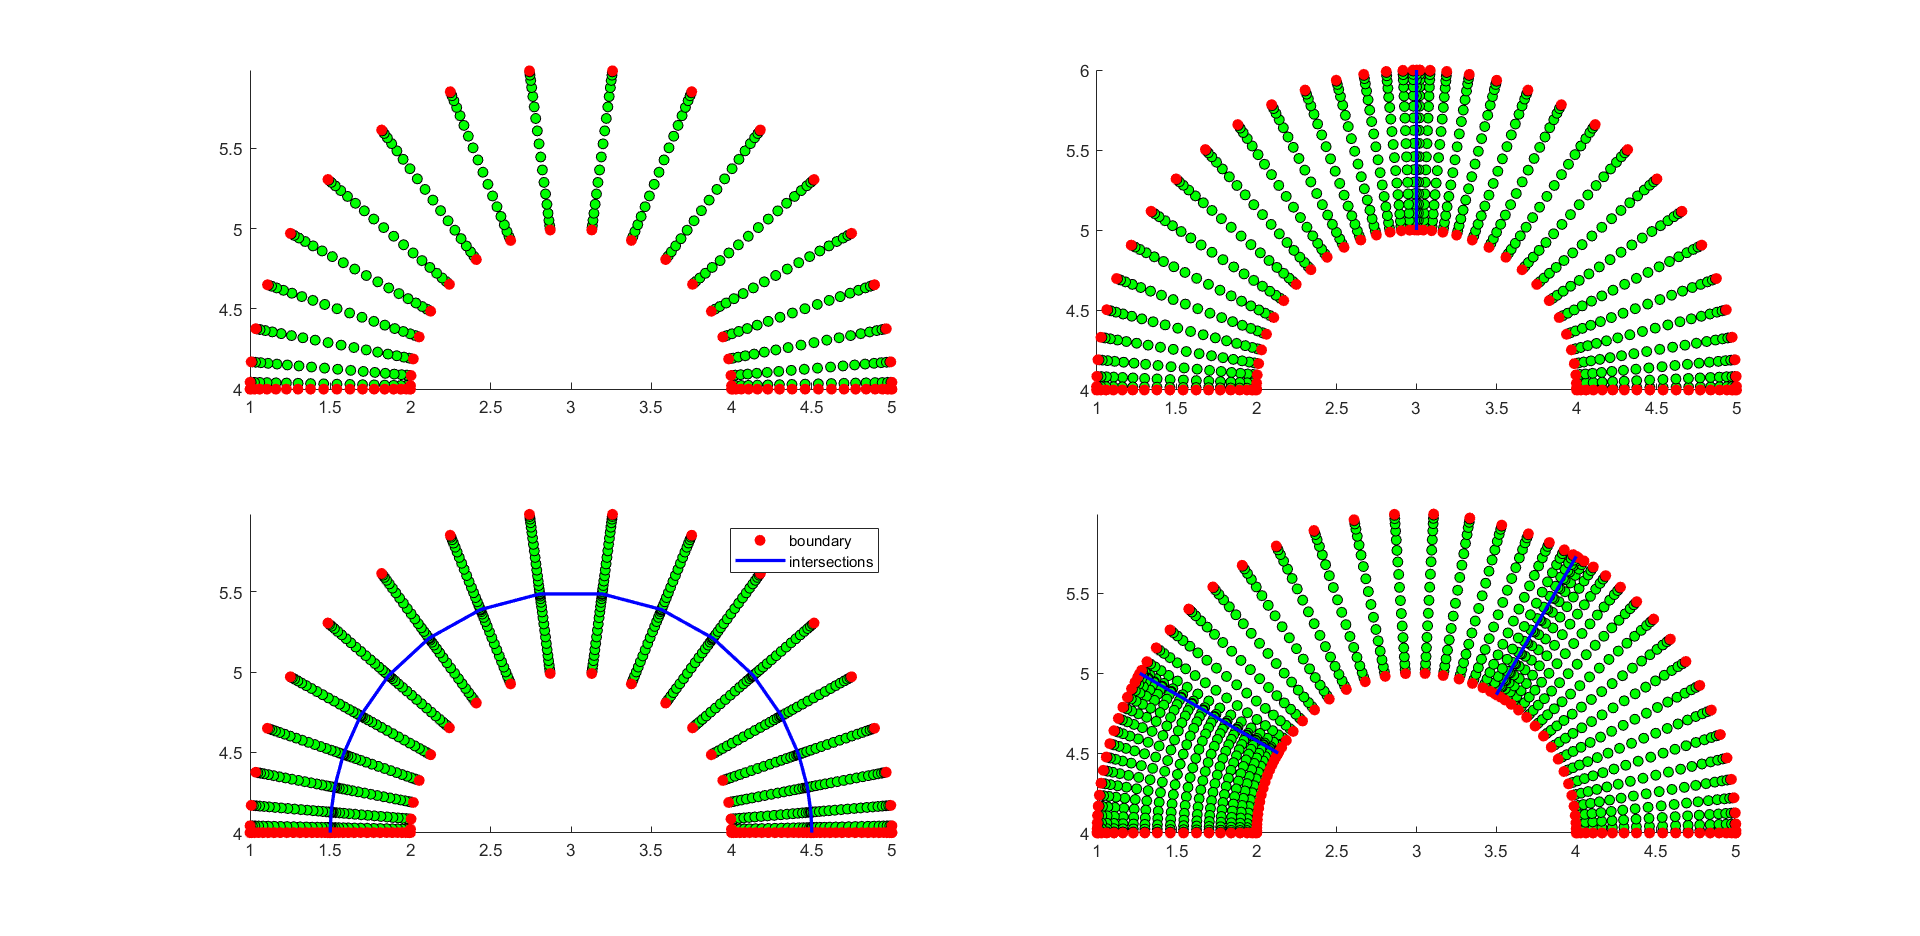
\includegraphics[scale=0.35]{WedgeSections.png}
	\caption{Different discretizations of the wedge (h -k).} 
	\label{F4}
\end{figure}





We investigate the accuracy of differentiation, interpolation, integration and convolution comparing different discretizations of the box and a wedge. The different discretizations can be seen in Figures \ref{F2}, \ref{F3a} and \ref{F4}.
The operations are validated using the exact solution
\begin{align}\label{eq:exactsol1}
	\rho &= \exp( \alpha_1  t + \beta_1 y_1 + \beta_2 y_2),\\
	\nabla \rho &= [\beta_1 \rho, \beta_2 \rho],\notag \\
	\nabla^2 \rho &= \nabla \cdot \nabla \rho = (\beta_1^2 + \beta_2^2)\rho,\notag
\end{align}
where $	\beta_1 = 0.1 $, $\beta_2 = 0.1$, $\alpha_1 = -0.5$.


We test each of the operators $\Grad$, $\Div$ and $\Lap$ by computing the error between the numerical and the exact solution
\begin{align}\label{eq:ErrorMeasure1}
	\mathcal E_{\text{Abs}} (f)&= \max \max \abs{f_{num} - f_{ex}}\\
	\mathcal E_{\text{Rel}} (f)&= \frac{\mathcal E_{\text{Abs}}(f) }{ \max \max \abs{f_{ex}}}.
\end{align}
The $\Div$ operator is tested by taking the divergence of the exact solution for $\nabla \rho$ and comparing it to the exact solution for $\nabla^2 \rho$. The solutions can be seen in Tables \ref{Tab:Grad}, \ref{Tab:div} and \ref{Tab:Lap}.
We investigate the functionality of the interpolation matrix by interpolating from the different multishapes onto a uniform grid. This grid is created by setting up a uniform rectangular grid which fully contains the multishape. Then we loop through the shapes and interpolate onto the uniform points that lie inside each shape. In the end we discard the points that lie outside the multishape. This causes the final solution on the uniform grid to vary in size, depending on the discretization of the multishape. We test the functionality by comparing the interpolated function values to the function evaluated on the uniform grid points, using \eqref{eq:ErrorMeasure1}. The results can be seen in Table \ref{Tab:Interp}.

We consider a similar approach for testing the convolution matrix. We compute the convolution with $N = 50$ on shape (a) (or (h) respectively) and apply it to the function $\rho$ in equation \eqref{eq:exactsol1}. We then interpolate this onto the other shapes and compute the error \eqref{eq:ErrorMeasure1} with the convolution of $\rho$ on that shape. We use the value of the convolution on a single shape with $N = 50$ as the reference value for the multishape convolution. The results are displayed in Table \ref{Tab:Conv}.

For the integration vector, we compute the integral of $\rho$ on shape (a) and compare this to the integral of $\rho$ on multishapes (b), (f) and (g). We then compare the integral of $\rho$ on the single shape (h) to the one on discretizations (j) and (k). The errors computed with \eqref{eq:ErrorMeasure1} can be seen in Table \ref{Tab:Int}, where again the value of the integral on the single shape is the reference for the multishape integration.
\begin{table}
\centering
\begin{tabular}{ | c | c | c | c | c | c | c |}
\hline
 & \multicolumn{2}{c|}{$N = 10$}  & \multicolumn{2}{c|}{$N = 20$}  & \multicolumn{2}{c|}{$N = 30$} \\
\hline
 & $\mathcal E_{Abs}$ & $\mathcal E_{Rel}$ & $\mathcal E_{Abs}$ & $\mathcal E_{Rel}$ & $\mathcal E_{Abs}$  & $\mathcal E_{Rel}$ \\
\hline
 a & $\numprint{3.6637e-15}$ & $\numprint{4.0491e-14}$ & $\numprint{4.5158e-14}$ & $\numprint{4.9908e-13}$ & $\numprint{1.0987e-13}$ & $\numprint{1.2143e-12}$ \\
 b & $\numprint{2.5202e-14}$ & $\numprint{2.7853e-13}$ & $\numprint{1.3006e-13}$ & $\numprint{1.4374e-12}$ & $\numprint{3.9264e-13}$ & $\numprint{4.3394e-12}$ \\
 c & $\numprint{3.5680e-14}$ & $\numprint{3.9432e-13}$ & $\numprint{2.7724e-13}$ & $\numprint{3.0639e-12}$ & $\numprint{1.0356e-12}$ & $\numprint{1.1445e-11}$ \\
 d & $\numprint{7.3080e-14}$ & $\numprint{8.0766e-13}$ & $\numprint{6.0429e-13}$ & $\numprint{6.6785e-12}$ & $\numprint{1.2559e-12}$ & $\numprint{1.3880e-11}$ \\
 e & $\numprint{3.1912e-14}$ & $\numprint{3.5268e-13}$ & $\numprint{2.0508e-13}$ & $\numprint{2.2665e-12}$ & $\numprint{6.5671e-13}$ & $\numprint{7.2578e-12}$ \\
 f & $\numprint{5.7149e-14}$ & $\numprint{6.3159e-13}$ & $\numprint{4.4410e-13}$ & $\numprint{4.9081e-12}$ & $\numprint{1.7717e-12}$ & $\numprint{1.9580e-11}$ \\
 g & $\numprint{1.3947e-14}$ & $\numprint{1.5414e-13}$ & $\numprint{9.5771e-14}$ & $\numprint{1.0584e-12}$ & $\numprint{2.6459e-13}$ & $\numprint{2.9242e-12}$ \\
 h & $\numprint{3.1143e-5}$ & $\numprint{1.3588e-4}$ & $\numprint{1.3522e-11}$ & $\numprint{5.9203e-11}$ & $\numprint{4.0515e-13}$ & $\numprint{1.7705e-12}$ \\
 i & $\numprint{1.3490e-7}$ & $\numprint{5.9567e-7}$ & $\numprint{2.4433e-13}$ & $\numprint{1.0689e-12}$ & $\numprint{4.5003e-13}$ & $\numprint{1.9658e-12}$ \\
 j & $\numprint{3.1143e-5}$ & $\numprint{1.3588e-4}$ & $\numprint{1.3522e-11}$ & $\numprint{5.9203e-11}$ & $\numprint{9.8901e-13}$ & $\numprint{4.3219e-12}$ \\
 k & $\numprint{9.8299e-8}$ & $\numprint{4.2888e-7}$ & $\numprint{3.1769e-13}$ & $\numprint{1.3866e-12}$ & $\numprint{8.6467e-13}$ & $\numprint{3.7732e-12}$ \\
\hline
\end{tabular}
\caption{Table $\Grad$}
\label{Tab:Grad}
\end{table}
\begin{table}
\centering
\begin{tabular}{ | c | c | c | c | c | c | c |}
\hline
 & \multicolumn{2}{c|}{$N = 10$}  & \multicolumn{2}{c|}{$N = 20$}  & \multicolumn{2}{c|}{$N = 30$} \\
\hline
 & $\mathcal E_{Abs}$ & $\mathcal E_{Rel}$ & $\mathcal E_{Abs}$ & $\mathcal E_{Rel}$ & $\mathcal E_{Abs}$  & $\mathcal E_{Rel}$ \\
\hline
 a & $\numprint{8.3267e-16}$ & $\numprint{4.6012e-14}$ & $\numprint{4.8798e-15}$ & $\numprint{2.6965e-13}$ & $\numprint{1.2278e-14}$ & $\numprint{6.7849e-13}$ \\
 b & $\numprint{2.9594e-15}$ & $\numprint{1.6353e-13}$ & $\numprint{1.3121e-14}$ & $\numprint{7.2507e-13}$ & $\numprint{4.0837e-14}$ & $\numprint{2.2566e-12}$ \\
 c & $\numprint{8.3614e-15}$ & $\numprint{4.6204e-13}$ & $\numprint{2.8682e-14}$ & $\numprint{1.5849e-12}$ & $\numprint{1.0649e-13}$ & $\numprint{5.8845e-12}$ \\
 d & $\numprint{7.9138e-15}$ & $\numprint{4.3731e-13}$ & $\numprint{4.2664e-14}$ & $\numprint{2.3575e-12}$ & $\numprint{9.6187e-14}$ & $\numprint{5.3152e-12}$ \\
 e & $\numprint{3.6846e-15}$ & $\numprint{2.0360e-13}$ & $\numprint{2.1975e-14}$ & $\numprint{1.2143e-12}$ & $\numprint{6.9682e-14}$ & $\numprint{3.8505e-12}$ \\
 f & $\numprint{9.7717e-15}$ & $\numprint{5.3997e-13}$ & $\numprint{6.4991e-14}$ & $\numprint{3.5913e-12}$ & $\numprint{1.3360e-13}$ & $\numprint{7.3824e-12}$ \\
 g & $\numprint{3.0878e-15}$ & $\numprint{1.7063e-13}$ & $\numprint{1.0623e-14}$ & $\numprint{5.8704e-13}$ & $\numprint{3.3662e-14}$ & $\numprint{1.8601e-12}$ \\
 h & $\numprint{5.2272e-5}$ & $\numprint{1.6127e-3}$ & $\numprint{3.4844e-11}$ & $\numprint{1.0758e-9}$ & $\numprint{5.3096e-14}$ & $\numprint{1.6387e-12}$ \\
 i & $\numprint{9.2692e-8}$ & $\numprint{2.8672e-6}$ & $\numprint{3.2897e-14}$ & $\numprint{1.0155e-12}$ & $\numprint{6.4497e-14}$ & $\numprint{1.9903e-12}$ \\
 j & $\numprint{5.2272e-5}$ & $\numprint{1.6127e-3}$ & $\numprint{3.4852e-11}$ & $\numprint{1.0761e-9}$ & $\numprint{1.3768e-13}$ & $\numprint{4.2490e-12}$ \\
 k & $\numprint{8.4307e-8}$ & $\numprint{2.6010e-6}$ & $\numprint{4.5634e-14}$ & $\numprint{1.4080e-12}$ & $\numprint{9.0605e-14}$ & $\numprint{2.7954e-12}$ \\
\hline
\end{tabular}
\caption{Table $\Div$}
\label{Tab:div}
\end{table}
\begin{table}
\centering
\begin{tabular}{ | c | c | c | c | c | c | c |}
\hline
 & \multicolumn{2}{c|}{$N = 10$}  & \multicolumn{2}{c|}{$N = 20$}  & \multicolumn{2}{c|}{$N = 30$} \\
\hline
 & $\mathcal E_{Abs}$ & $\mathcal E_{Rel}$ & $\mathcal E_{Abs}$ & $\mathcal E_{Rel}$ & $\mathcal E_{Abs}$  & $\mathcal E_{Rel}$ \\
\hline
 a & $\numprint{1.7055e-13}$ & $\numprint{9.4244e-12}$ & $\numprint{4.7951e-12}$ & $\numprint{2.6497e-10}$ & $\numprint{2.5029e-11}$ & $\numprint{1.3831e-9}$ \\
 b & $\numprint{1.3937e-12}$ & $\numprint{7.7015e-11}$ & $\numprint{4.4301e-11}$ & $\numprint{2.4480e-9}$ & $\numprint{1.2869e-10}$ & $\numprint{7.1114e-9}$ \\
 c & $\numprint{7.7744e-12}$ & $\numprint{4.2960e-10}$ & $\numprint{3.8083e-10}$ & $\numprint{2.1044e-8}$ & $\numprint{3.8902e-9}$ & $\numprint{2.1497e-7}$ \\
 d & $\numprint{1.4964e-11}$ & $\numprint{8.2688e-10}$ & $\numprint{5.5707e-10}$ & $\numprint{3.0783e-8}$ & $\numprint{1.6726e-9}$ & $\numprint{9.2426e-8}$ \\
 e & $\numprint{4.2647e-12}$ & $\numprint{2.3566e-10}$ & $\numprint{1.0580e-10}$ & $\numprint{5.8462e-9}$ & $\numprint{1.0035e-9}$ & $\numprint{5.5450e-8}$ \\
 f & $\numprint{1.4029e-11}$ & $\numprint{7.7521e-10}$ & $\numprint{5.8611e-10}$ & $\numprint{3.2388e-8}$ & $\numprint{3.0143e-9}$ & $\numprint{1.6657e-7}$ \\
 g & $\numprint{9.4664e-13}$ & $\numprint{5.2310e-11}$ & $\numprint{3.5819e-11}$ & $\numprint{1.9793e-9}$ & $\numprint{1.4403e-10}$ & $\numprint{7.9586e-9}$ \\
 h & $\numprint{5.3665e-4}$ & $\numprint{1.6556e-2}$ & $\numprint{1.0457e-9}$ & $\numprint{3.2287e-8}$ & $\numprint{1.7551e-10}$ & $\numprint{5.4167e-9}$ \\
 i & $\numprint{4.6482e-6}$ & $\numprint{1.4378e-4}$ & $\numprint{5.0420e-11}$ & $\numprint{1.5565e-9}$ & $\numprint{2.3952e-10}$ & $\numprint{7.3915e-9}$ \\
 j & $\numprint{5.3665e-4}$ & $\numprint{1.6556e-2}$ & $\numprint{1.0223e-9}$ & $\numprint{3.1565e-8}$ & $\numprint{7.2370e-10}$ & $\numprint{2.2335e-8}$ \\
 k & $\numprint{3.3996e-6}$ & $\numprint{1.0488e-4}$ & $\numprint{1.0291e-10}$ & $\numprint{3.1753e-9}$ & $\numprint{4.0443e-10}$ & $\numprint{1.2478e-8}$ \\
\hline
\end{tabular}
\caption{Table $\Lap$}
\label{Tab:Lap}
\end{table}
\begin{table}
\centering
\begin{tabular}{ | c | c | c | c | c | c | c |}
\hline
 & \multicolumn{2}{c|}{$N = 10$}  & \multicolumn{2}{c|}{$N = 20$}  & \multicolumn{2}{c|}{$N = 30$} \\
\hline
 & $\mathcal E_{Abs}$ & $\mathcal E_{Rel}$ & $\mathcal E_{Abs}$ & $\mathcal E_{Rel}$& $\mathcal E_{Abs}$  & $\mathcal E_{Rel}$ \\
\hline
 a & $\numprint{9.9920e-16}$ & $\numprint{1.1043e-15}$ & $\numprint{1.1102e-15}$ & $\numprint{1.2270e-15}$ & $\numprint{1.9984e-15}$ & $\numprint{2.2086e-15}$ \\
 b & $\numprint{8.8818e-16}$ & $\numprint{9.8159e-16}$ & $\numprint{1.5543e-15}$ & $\numprint{1.7178e-15}$ & $\numprint{1.8874e-15}$ & $\numprint{2.0859e-15}$ \\
 c & $\numprint{8.8818e-16}$ & $\numprint{9.8159e-16}$ & $\numprint{1.6653e-15}$ & $\numprint{1.8405e-15}$ & $\numprint{2.2204e-15}$ & $\numprint{2.4540e-15}$ \\
 d & $\numprint{8.8818e-16}$ & $\numprint{9.8159e-16}$ & $\numprint{1.9984e-15}$ & $\numprint{2.2086e-15}$ & $\numprint{2.6645e-15}$ & $\numprint{2.9448e-15}$ \\
 e & $\numprint{8.8818e-16}$ & $\numprint{9.8159e-16}$ & $\numprint{1.4433e-15}$ & $\numprint{1.5951e-15}$ & $\numprint{2.6645e-15}$ & $\numprint{2.9448e-15}$ \\
 f & $\numprint{1.2212e-15}$ & $\numprint{1.3497e-15}$ & $\numprint{1.6653e-15}$ & $\numprint{1.8405e-15}$ & $\numprint{2.8866e-15}$ & $\numprint{3.1902e-15}$ \\
 g & $\numprint{8.8818e-16}$ & $\numprint{9.8159e-16}$ & $\numprint{1.8874e-15}$ & $\numprint{2.0859e-15}$ & $\numprint{2.5535e-15}$ & $\numprint{2.8221e-15}$ \\
 h & $\numprint{4.6655e-6}$ & $\numprint{2.8922e-6}$ & $\numprint{7.9314e-13}$ & $\numprint{4.9000e-13}$ & $\numprint{2.6645e-15}$ & $\numprint{1.6450e-15}$ \\
 i & $\numprint{1.1935e-8}$ & $\numprint{7.3650e-9}$ & $\numprint{3.3307e-15}$ & $\numprint{2.0553e-15}$ & $\numprint{3.1086e-15}$ & $\numprint{1.9183e-15}$ \\
 j & $\numprint{4.6655e-6}$ & $\numprint{2.8922e-6}$ & $\numprint{7.9226e-13}$ & $\numprint{4.8945e-13}$ & $\numprint{4.2188e-15}$ & $\numprint{2.6047e-15}$ \\
 k & $\numprint{7.7730e-9}$ & $\numprint{4.8017e-9}$ & $\numprint{2.2204e-15}$ & $\numprint{1.3705e-15}$ & $\numprint{4.4409e-15}$ & $\numprint{2.7405e-15}$ \\
\hline
\end{tabular}
\caption{Table Interp}
\label{Tab:Interp}
\end{table}
\begin{table}
\centering
\begin{tabular}{ | c | c || c | c | c | c | c ||}
\hline
 & A.E. $ N=10$ & R.E. $N=10$ & A.E. $N = 20$ & R.E. $N = 20$ & A.E. $N=30$  & R.E. $N=30$ \\
\hline
\hline
 b & $\numprint{9.1924e-8}$ & $\numprint{5.5907e-8}$ & $\numprint{7.5495e-15}$ & $\numprint{4.5500e-15}$ & $\numprint{8.2157e-15}$ & $\numprint{4.9463e-15}$ \\
 f & $\numprint{1.4109e-8}$ & $\numprint{8.5341e-9}$ & $\numprint{8.2157e-15}$ & $\numprint{4.9497e-15}$ & $\numprint{1.9984e-14}$ & $\numprint{1.2033e-14}$ \\
 g & $\numprint{1.9228e-10}$ & $\numprint{1.1579e-10}$ & $\numprint{9.7700e-15}$ & $\numprint{5.8815e-15}$ & $\numprint{1.5543e-14}$ & $\numprint{9.3564e-15}$ \\
 j & $\numprint{1.6310e-3}$ & $\numprint{6.6333e-4}$ & $\numprint{5.0919e-8}$ & $\numprint{2.0616e-8}$ & $\numprint{8.9782e-12}$ & $\numprint{3.6342e-12}$ \\
 k & $\numprint{2.7196e-6}$ & $\numprint{1.1056e-6}$ & $\numprint{1.7668e-12}$ & $\numprint{7.1588e-13}$ & $\numprint{2.9310e-14}$ & $\numprint{1.1870e-14}$ \\
\hline
\end{tabular}
\caption{Table Conv}
\label{Tab:Conv}
\end{table}
\begin{table}
\centering
\begin{tabular}{ | c | c || c | c | c | c | c ||}
\hline
 & A.E. $ N=10$ & R.E. $N=10$ & A.E. $N = 20$ & R.E. $N = 20$ & A.E. $N=30$  & R.E. $N=30$ \\
\hline
\hline
 b & $\numprint{0.0000e+00}$ & $\numprint{0.0000e+00}$ & $\numprint{4.4409e-16}$ & $\numprint{1.4937e-16}$ & $\numprint{8.8818e-16}$ & $\numprint{2.9873e-16}$ \\
 f & $\numprint{0.0000e+00}$ & $\numprint{0.0000e+00}$ & $\numprint{0.0000e+00}$ & $\numprint{0.0000e+00}$ & $\numprint{8.8818e-16}$ & $\numprint{2.9873e-16}$ \\
 g & $\numprint{0.0000e+00}$ & $\numprint{0.0000e+00}$ & $\numprint{4.4409e-16}$ & $\numprint{1.4937e-16}$ & $\numprint{8.8818e-16}$ & $\numprint{2.9873e-16}$ \\
 j & $\numprint{2.4085e-8}$ & $\numprint{3.7621e-9}$ & $\numprint{1.7764e-15}$ & $\numprint{2.7746e-16}$ & $\numprint{2.6645e-15}$ & $\numprint{4.1620e-16}$ \\
 k & $\numprint{2.7334e-11}$ & $\numprint{4.2695e-12}$ & $\numprint{1.7764e-15}$ & $\numprint{2.7746e-16}$ & $\numprint{1.7764e-15}$ & $\numprint{2.7746e-16}$ \\
\hline
\end{tabular}
\caption{Table Int}
\label{Tab:Int}
\end{table}

\section{Exact Tests}
The solution to known testproblems with Dirichlet and no-flux boundary conditions are considered in this section. The errors are calculated as an $l_2$ error in space and an $l_\infty$ error in time.
\subsection{Exact Tests - Dirichlet Conditions}
(MS\_TestJonnaADExactDisectBoxes and MS\_TestJonnaADExactDisectBoxesPart2\\ and MS\_TestJonnaADExactDisectWedges)
Several examples are run, using exact solutions, to validate the multishape code. This is done using an exact solution to the advection diffusion equation on an infinite domain, so that Dirichlet boundary conditions, matching the value of the exact solution on the boundary of the multishape, can be applied.
The exact solution is \cite{Hutomo_2019}
\begin{align*}
	\rho &= \exp(\alpha t + \beta_1 y_1 + \beta_2 y_2)\\
	\mathbf v &= \left(\beta_1 - \frac{\alpha}{2 \beta_1} + p_1\exp(-\beta_1 y_1) , \beta_2 - \frac{\alpha}{2 \beta_2} + p_2\exp(-\beta_2 y_2) \right),
\end{align*}
where $\beta_1 = 0.1$, $\beta_2 = 0.1$, $\alpha = -0.5$, $p_1 = -1$ and $p_2 = 1$.
We compare the exact solution on a box of dimensions $[0,2] \times [0,2] $ with different discretizations of the box using multishape, see Figure \ref{F2}. Each of the shapes are discretized with $N = 10$, $N = 20$ and $N = 30$ points in each spatial direction, which means that the dissected box has more points in total than the original box. The ODE solver tolerances are $10^{-9}$. The solution can be seen in Figure \ref{F3}. The question is whether the results of the PDE on the box and the different discretizations of the box have a similar error when compared to the exact solution. The absolute and relative errors are measured in an $l_2$ norm in space and an $l_\infty$ norm in time and are displayed in Table \ref{Tab1:ErrorsExBox}. The bottom row contains errors for the non-rectangular quadrilateral, which is shown in Figure \ref{F3a}. 
\begin{table}
	\begin{tabular}{ ||c| c| c| c| c |c|c|| }
		\hline
		\hline
		& A.E. $N =10$ & R.E. $N =10$ &A.E. $N =20$ & R.E. $N =20$ &A.E. $N =30$ & R.E. $N =30$ \\ 
		\hline
		a & $2.5869 \times 10^{-7}$ & $1.0894 \times 10^{-9}$ & $2.2063 \times 10^{-7}$ & $1.1235 \times 10^{-9}$ & $2.1913 \times 10^{-7}$ & $1.1159 \times 10^{-9}$ \\  
		b & $3.4991\times 10^{-7}$ & $1.1308 \times 10^{-9}$ &  $3.2073 \times 10^{-7}$ & $1.1377 \times 10^{-9}$  & $3.1878 \times 10^{-7}$ & $1.1308 \times 10^{-9}$\\  
		c & $4.1386\times 10^{-7}$  & $1.1596 \times 10^{-9}$ & $3.9108\times 10^{-7}$ & $1.15 \times 10^{-9}$  & $3.8859\times 10^{-7}$ & $1.1427\times 10^{-9}$ \\  
		d & $4.2622\times 10^{-7}$ & $1.0268 \times 10^{-9} $& $3.902\times 10^{-7}$ & $1.0026 \times 10^{-9}$ & $3.8767\times 10^{-7}$ & $9.9612 \times 10^{-10}$\\
		e & $4.1985 \times 10^{-7}$ & $1.0275 \times 10^{-9}$  & $4.2546 \times 10^{-7}$ & $1.0412 \times 10^{-9}$  & $4.2292 \times 10^{-7}$  & $1.035 \times 10^{-9}$ \\
		f & $4.4594 \times 10^{-7}$  & $1.0704 \times 10^{-9}$ & $3.3849 \times 10^{-7}$ & $9.8249 \times 10^{-10}$&  $3.3719 \times 10^{-7}$&  $1.0085 \times 10^{-9}$\\
		g & $5.0161\times 10^{-7}$ & $1.1254 \times 10^{-9}$  & $4.4469\times 10^{-7}$& $1.1323 \times 10^{-9}$ &  $4.3978\times 10^{-7}$& $1.1198\times 10^{-9}$\\
		q & $2.4145\times 10^{-7}$ & $1.0389\times 10^{-9}$ & $2.2844\times 10^{-7}$ & $1.116\times 10^{-9}$ & $2.2505\times 10^{-7}$ & $1.0995\times 10^{-9}$\\
		\hline
		\hline
	\end{tabular}
	\caption{Errors in the Dirichlet forward problem compared to exact solution for different discretizations of the box and a quadrilateral (absolute error A.E. and relative error R.E. are compared)}
	\label{Tab1:ErrorsExBox}
\end{table}

	\begin{figure}[h]
		\centering
		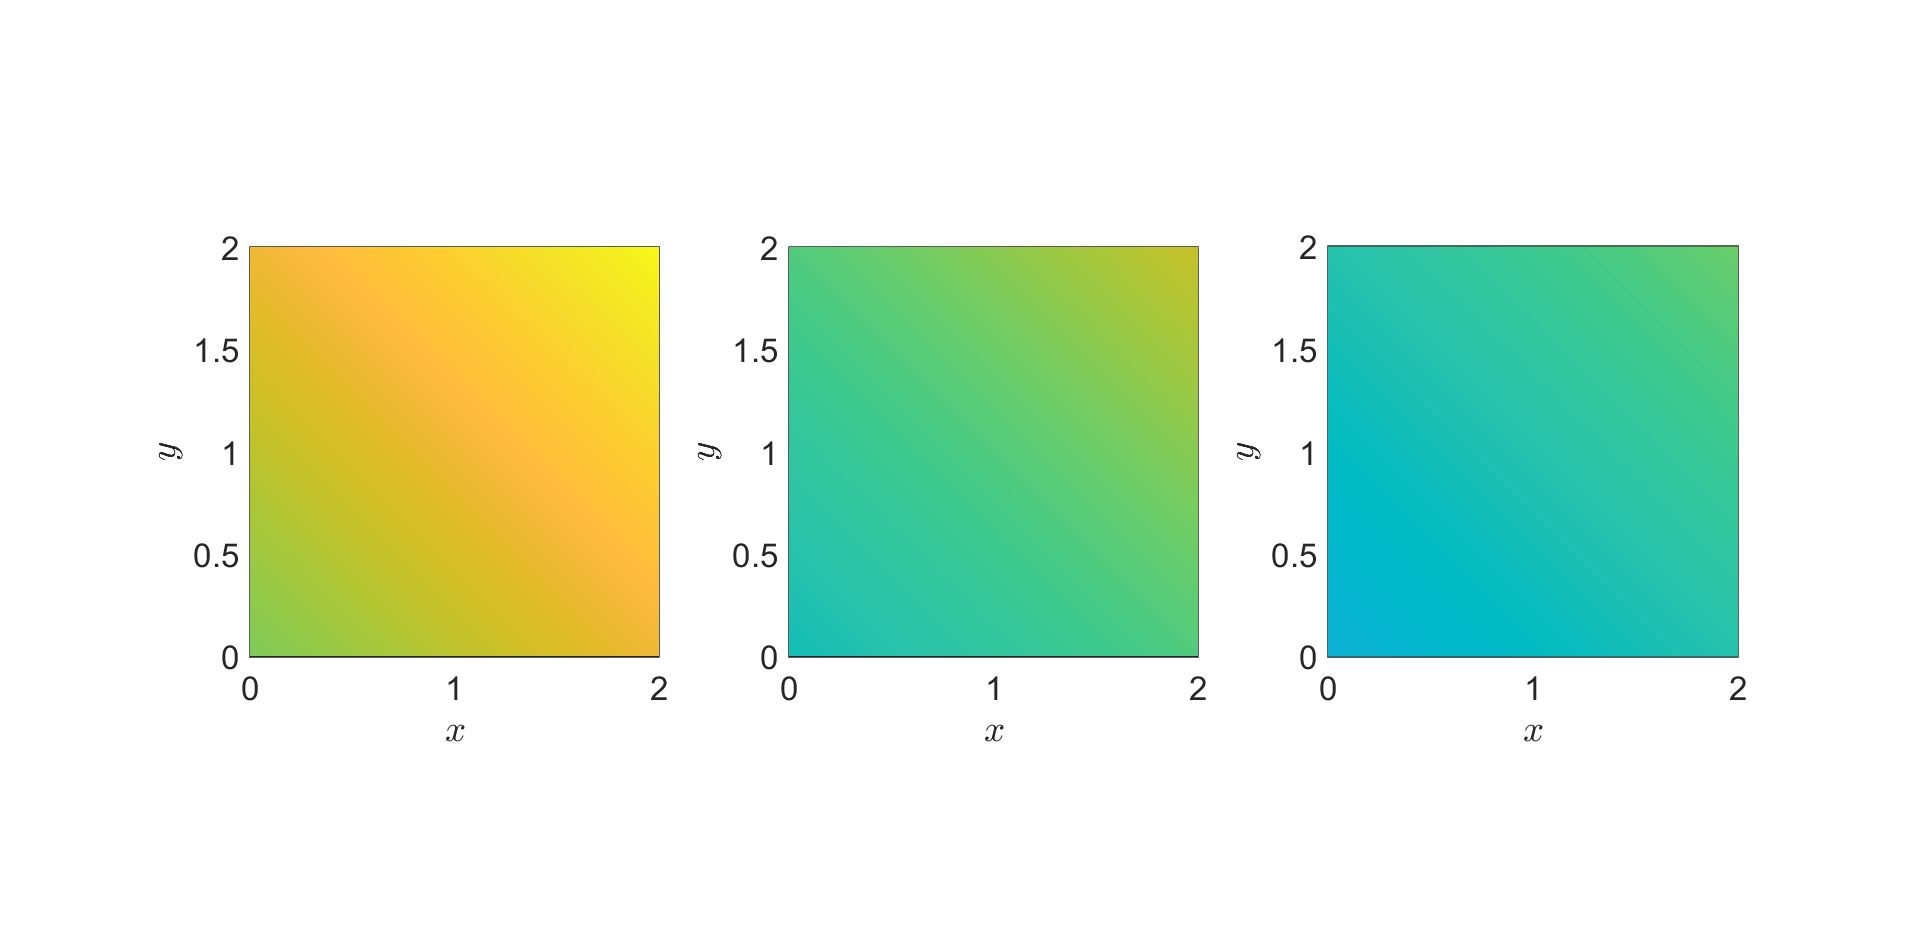
\includegraphics[scale=0.35]{boxEx.png}
		\caption{Exact solution on the box.} 
		\label{F3}
	\end{figure}


The same test can be done for a wedge. Here, a single wedge and discretized versions are considered, see Figure \ref{F4}. Table \ref{Tab2:ErrorsExWedge} shows the errors measured against the exact solution for different discretizations of the wedge for $N = 10$, $N = 20$ and $N = 30$. The solution can be seen in Figure \ref{F5}.


\begin{figure}[h]
	\centering
	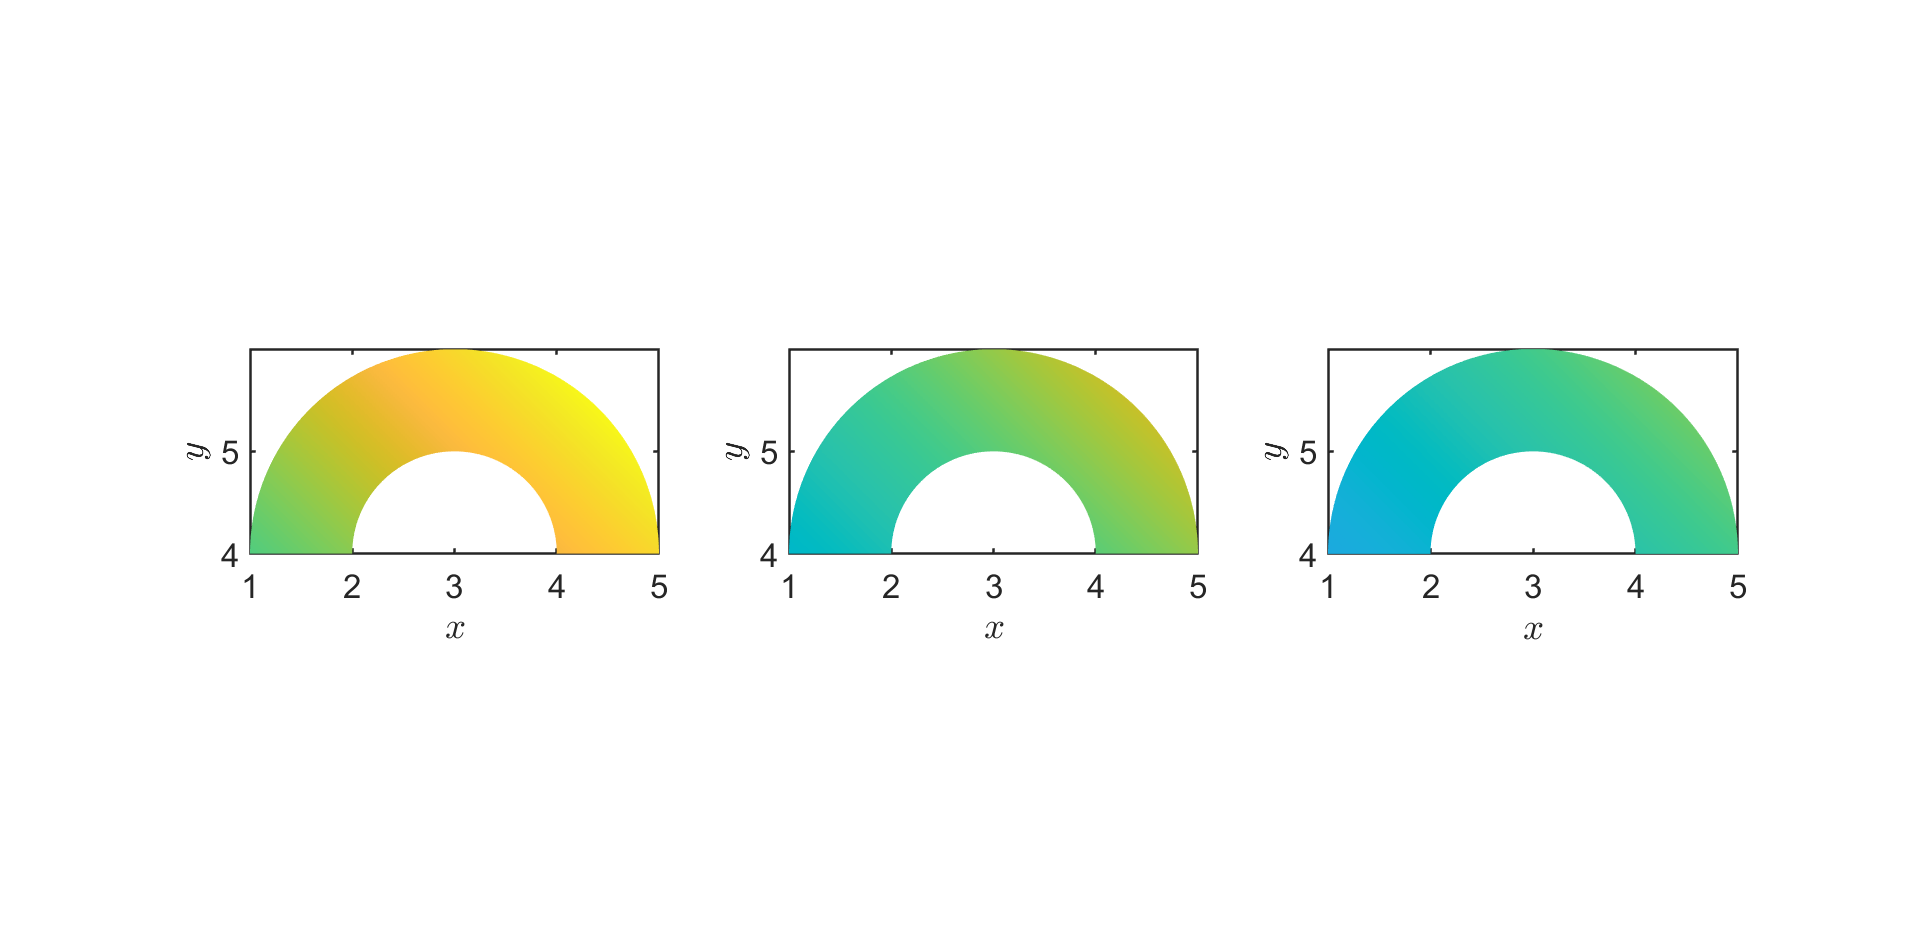
\includegraphics[scale=0.35]{wedgeEx.png}
	\caption{Exact solution on the wedge.} 
	\label{F5}
\end{figure}
\begin{table}
	\caption{Errors compared to exact solution for different discretization (into one, two and three shapes) of the wedge}
	\begin{tabular}{ ||c| c| c| c| c|| }
		\hline
		\hline
		& h & i & j& k\\ 
		\hline
		Abs. Error, $N =10$& $0.0019$ & $3.4678 \times 10^{-6}$ & $0.0026$ & $2.6814\times 10^{-6}$\\  
		Rel. Error, $N =10$& $4.441 \times 10^{-6}$& $6.5183 \times 10^{-9}$ &$4.4489 \times 10^{-6}$ &  $4.0877\times 10^{-9}$\\
		\hline
		Abs. Error, $N =20$& $3.1141 \times 10^{-7}$ & $3.9526 \times 10^{-7}$ & $4.2335\times 10^{-7}$ & $4.4145\times 10^{-7}$\\  
		Rel. Error, $N =20$& $7.4762 \times 10^{-10}$& $7.5984 \times 10^{-10}$ &$7.4942 \times 10^{-10}$ &  $7.0897 \times 10^{-10}$\\
		\hline
		Abs. Error, $N =30$& $ 2.7613\times 10^{-7}$ & $ 3.8484\times 10^{-7}$ & $3.892\times 10^{-7}$ & $4.3211\times 10^{-7}$ \\  
		Rel. Error, $N =30$ & $ 7.5178\times 10^{-10}$& $ 7.4375\times 10^{-10}$ &$7.5061\times 10^{-10}$ & $6.9683\times 10^{-10}$  \\
		\hline
		\hline
	\end{tabular}
	\label{Tab2:ErrorsExWedge}
\end{table}
Next the advection diffusion equation is solved on a multishape which is composed of four quadrilaterals, see Figure \ref{F6}. The absolute error for $N = 20$ on each shape as compared to the exact solution is $6.1246 \times 10^{-7}$ and the relative error is $1.3259 \times 10^{-9}$. 
\begin{figure}[h]
	\centering
	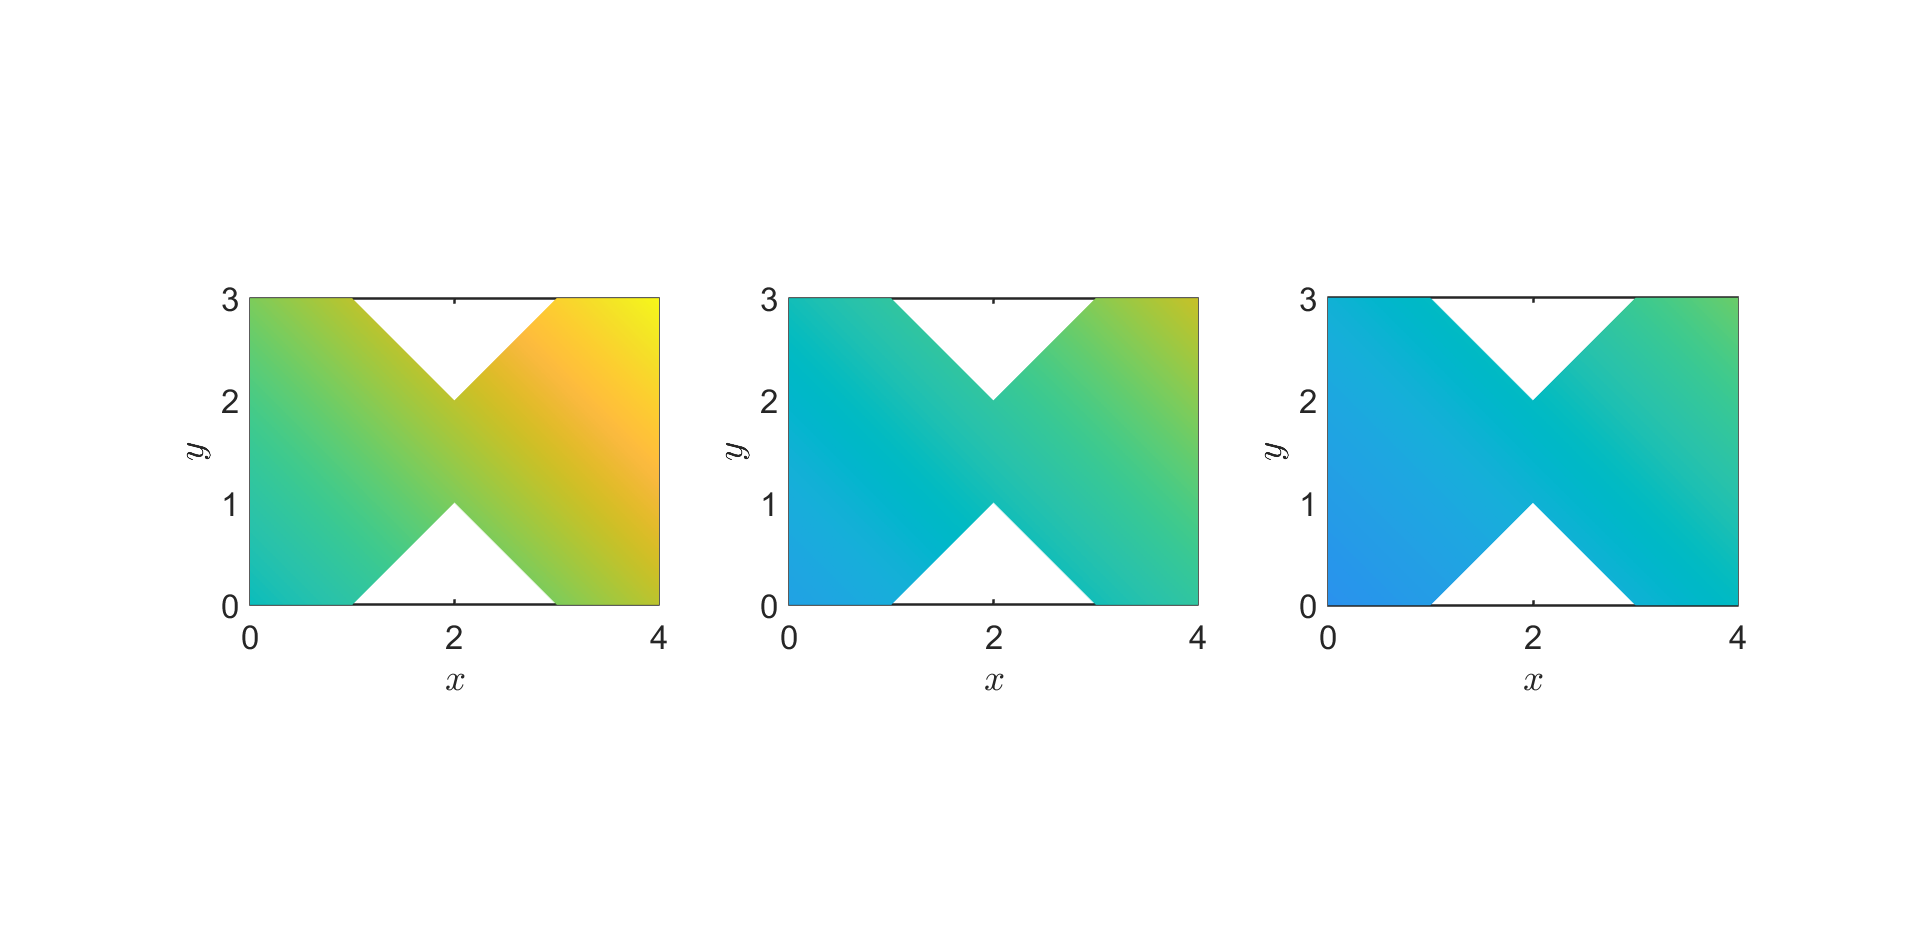
\includegraphics[scale=0.35]{example1.png}
	\caption{Example 1 multishape} 
	\label{F6}
\end{figure}
The same is done for a second example involving a wedge, see Figure \ref{F7}. The absolute error to the exact solution is $3.7239 \times 10^{-7}$ and the relative error is $8.9375 \times 10^{-10}$, when choosing $N= 20$ per shape. 

\begin{figure}[h]
	\centering
	\includegraphics[scale=0.35]{example2.png}
	\caption{Example 2 multishape} 
	\label{F7}
\end{figure}


\subsection{Exact Tests - Dirichlet Conditions, Solution 2}

We solve an exact Dirichlet problem which does not have an exponential form but a quadratic form. In order to do this, we add on a source term $f$ to the advection-diffusion equation.
We define the exact solution as
\begin{align*}
	\rho &= t y_1^2 y_2^2,\\
	f &= y_1^2 y_2^2 - 2 y_1^2 t - 2 y_2^2 t + 2 y_1 y_2^2 t,
\end{align*}
and with a velocity field of strength one acting in the $y_1$ direction.
We run this on a few of the problems on the box and the wedge (a,b,c,f, h, j, k). The results are displayed in Table \ref{Tab4}.

\begin{table}
	\caption{Errors for discretization of the box and wedge for a quadratic exact Dirichlet solution}
	\begin{tabular}{ ||c| c| c| c| c |c|c|| }
		\hline
		\hline
		& A.E. $N =10$ & R.E. $N =10$ &A.E. $N =20$ & R.E. $N =20$ &A.E. $N =30$ & R.E. $N =30$ \\ 
		\hline
		a & $ 2.2747\times 10^{-13 }$ & $ 3.9799\times 10^{-16 }$ & $ 3.9207\times 10^{-13 }$ & $6.3023 \times 10^{-16 }$ & $4.7291 \times 10^{- 13}$ & $ 7.5978\times 10^{-16 }$\\  
		b & $ 1.1317\times 10^{-12 }$ & $1.1097 \times 10^{-15}$ & $6.1443 \times 10^{-13 }$ & $ 5.985\times 10^{-16 }$ & $2.5646 \times 10^{- 12}$ & $2.5682 \times 10^{-15 }$\\  
		c & $ 7.0072\times 10^{- 13}$ & $ 7.0033 \times 10^{-16 }$ & $1.4084 \times 10^{-12 }$ & $ 1.3513\times 10^{- 15}$ & $2.0691 \times 10^{- 12}$ & $ 2.4102\times 10^{-15 }$\\  
		f & $ 8.2166\times 10^{- 13}$ & $1.6362\times 10^{- 15} $ & $ 1.5548 \times 10^{-12 } $ & $1.0522 \times 10^{-15 }$ & $2.6986 \times 10^{-12} $ & $ 1.7149\times 10^{- 15}$\\  
	    \hline
		h & $0.0262 $ & $3.1608 \times 10^{-7}$ & $ 5.9536\times 10^{- 11}$ & $7.4829 \times 10^{-16 }$ & $ 8.2469\times 10^{-11}$ & $ 1.0421\times 10^{-15}$\\  
		j & $13.0821 $ & $0.0002 $ & $ 5.1279 \times 10^{- 6}$ & $6.1963 \times 10^{-11 }$ & $2.1582 \times 10^{- 10}$ & $ 2.7077\times 10^{-15}$\\  
		k & $0.0193$ & $ 2.0145\times 10^{- 7}$ & $6.8171 \times 10^{-11 }$ & $ 7.4486\times 10^{-16 }$ & $ 9.9529 \times 10^{-11}$ & $ 1.0842\times 10^{-15}$\\  
		\hline
		\hline
	\end{tabular}
	\label{Tab4}
\end{table}

\subsection{Exact Tests - No-Flux Conditions}
We consider an exact solution on a box with no-flux boundary conditions for the advection diffusion equation. The solution is
\begin{align*}
	 \rho = 2 + \exp(-(\mu_1^2 + \mu_2^2)t)\cos(\mu_1 y_1)\cos(\mu_2 y_2),
\end{align*}
where $	\mu_1 = n\pi/L_1$, $\mu_2 = n\pi/L_2$ and $n = 2$, $L_1 = d - c$, $ L_2 = b - a$ for a domain $ [a,b]\times [c,d]$. We use the discretizations of the box displayed in Figure \ref{F2} with $N = 10$, $N= 20$ and $N = 30$. The exact solution for this problem can be seen in Figure \ref{F3b}. In Table \ref{Tab3:ErrorsNoFlux} we can see the errors made on the different discretizations. We can observe that the errors in multishapes (c), (d) and (f) are considerably larger than the errors for the other shapes. This is because of the complex discretization chosen in these multishapes. Due to this discretization, the standard averaging of the two normals at an intersection corner does not result in reasonable normals, see Figure \ref{FNorm}. This becomes an issue when computing no-flux boundary conditions, since this needs the normal information. The code library offers the option of overriding individual normals. We redefine the normals at the intersection corner to be the outward normals of the box. This improves the errors greatly as can be seen in Table \ref{Tab3:ErrorsNoFlux2}.

\begin{figure}[h]
	\centering
	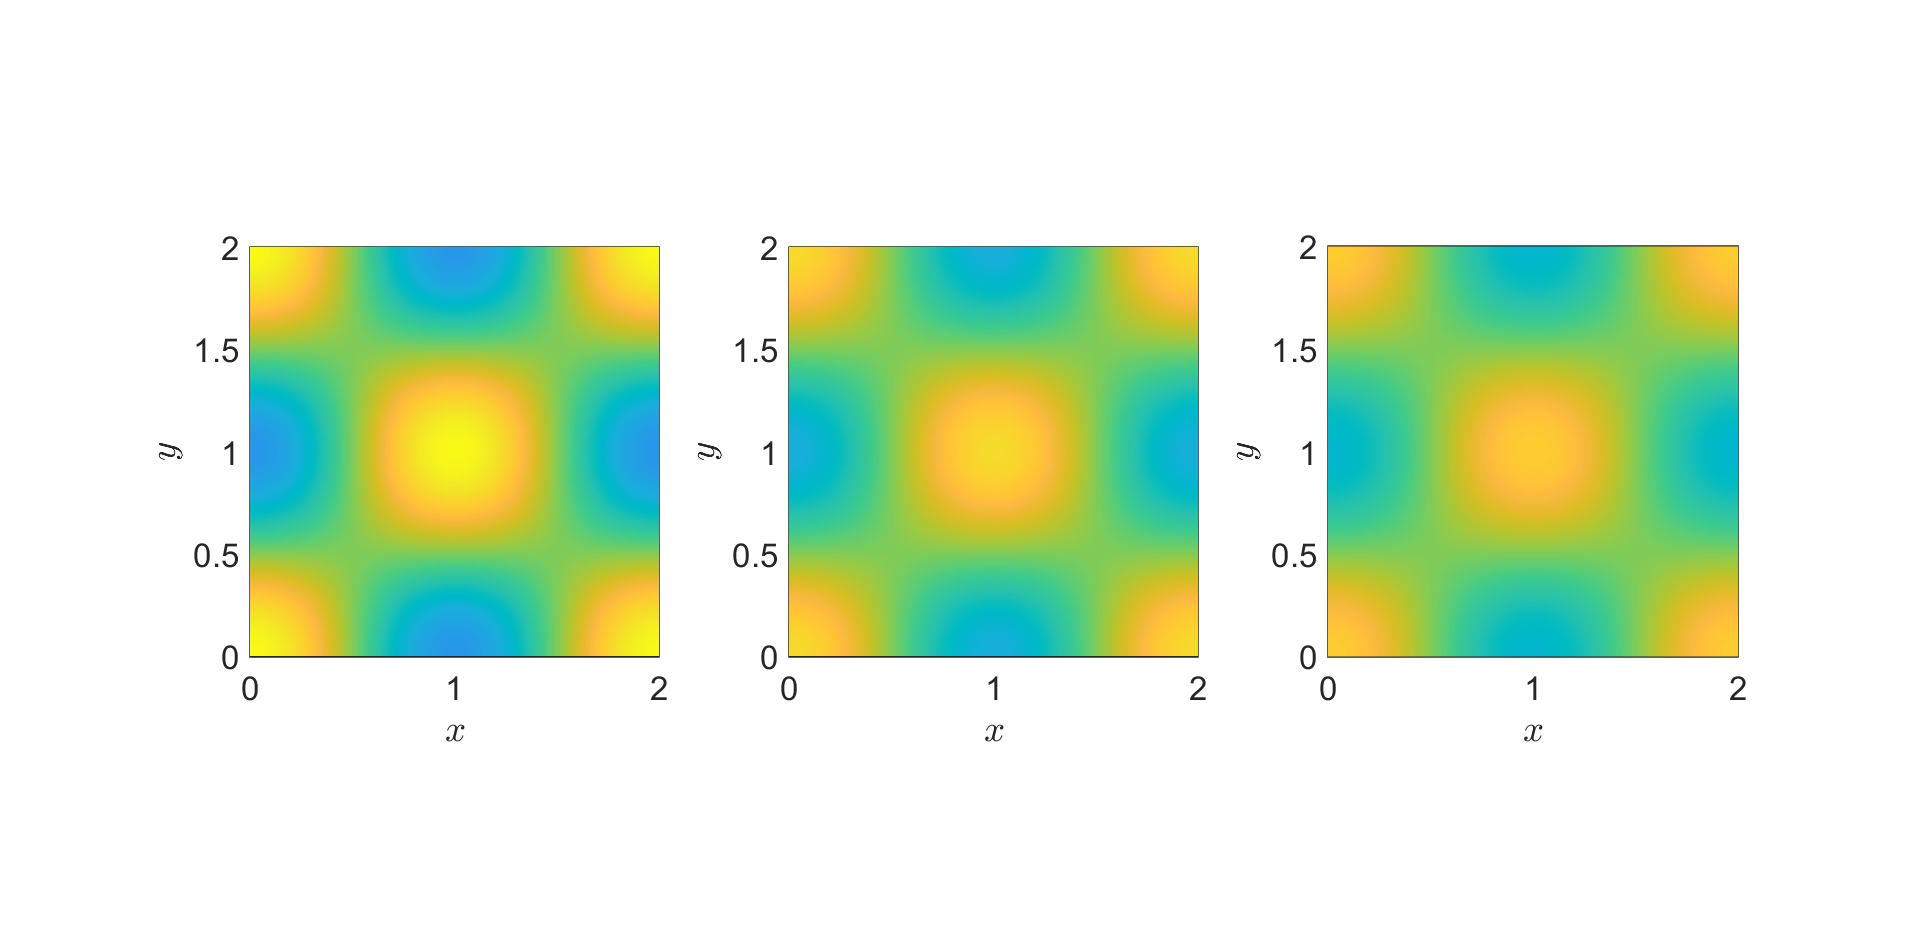
\includegraphics[scale=0.35]{boxExNoFlux.png}
	\caption{Exact solution on the box with no-flux boundary conditions.} 
	\label{F3b}
\end{figure}
\begin{table}
	\caption{Errors compared to exact solution with no-flux boundary conditions for different discretization of the box (absolute error A.E. and relative error R.E. are compared)}
	\begin{tabular}{ ||c| c| c| c| c |c|c|| }
		\hline
		\hline
		& A.E. $N =10$ & R.E. $N =10$ &A.E. $N =20$ & R.E. $N =20$ &A.E. $N =30$ & R.E. $N =30$ \\ 
		\hline
		a & $0.0105$ & $2.523 \times 10^{-5}$ & $2.8349\times 10^{-7}$ & $6.862\times 10^{-10}$ & $2.682\times 10^{-7}$ & $6.4921\times 10^{-10}$\\  
		b & $0.0102$ & $1.7387\times 10^{-5}$ & $3.5488\times 10^{-7}$ & $6.0816\times 10^{-10}$ & $3.5538\times 10^{-7}$ & $6.0901\times 10^{-10}$\\  
		c & $0.0713$ & $9.8994 \times 10^{-5}$ & $0.0070$ & $9.7842\times 10^{-6}$ & $0.0026$ & $3.6463\times 10^{-6}$\\  
		d & $0.0849$ & $0.0001               $ & $0.0083$ & $9.9356\times 10^{-6}$ & $0.0030$ & $3.6506\times 10^{-6}$\\  
		e & $0.0057$ & $8.1264 \times 10^{-6}$ & $4.3058\times 10^{-7}$ & $6.0667\times 10^{-10}$ & $4.3145\times 10^{-7}$ & $6.0789\times 10^{-10}$\\  
		f & $0.1293$ & $0.0002$ & $0.0135$ & $1.6099\times 10^{-5}$ & $0.0040$ & $4.8753\times 10^{-6}$\\  
		g & $8.7462 \times 10^{-6}$ & $1.0753\times 10^{-8}$ & $5.1503\times 10^{-7}$ & $6.2334\times 10^{-10}$ & $5.147\times 10^{-7}$ & $6.2295\times 10^{-10}$\\  
		\hline
		\hline
	\end{tabular}
	\label{Tab3:ErrorsNoFlux}
\end{table}

\begin{table}
	\caption{Errors compared to exact solution with no-flux boundary conditions for multishapes (c), (d) and (f) after correcting the normal vectors (absolute error A.E. and relative error R.E. are compared)}
	\begin{tabular}{ ||c| c| c| c| c |c|c|| }
		\hline
		\hline
		& A.E. $N =10$ & R.E. $N =10$ &A.E. $N =20$ & R.E. $N =20$ &A.E. $N =30$ & R.E. $N =30$ \\ 
		\hline
		c & $0.0187$ & $2.5911 \times 10^{-5}$ & $4.5961 \times 10^{-7}$ & $6.4023 \times 10^{-10}$ & $4.5881 \times 10^{-7} $ & $6.3911 \times 10^{-10}$\\  
		d & $0.0243$ & $2.9194 \times 10^{-5} $ & $5.2874 \times 10^{-7} $ & $6.381 \times 10^{-10}$ & $5.2815 \times 10^{-7} $ & $6.374 \times 10^{-10}$\\  
		f & $0.0022$ & $2.6634 \times 10^{-6}$ & $ 5.3703 \times 10^{-7}$ & $ 6.3964\times 10^{-10}$ & $ 5.3681 \times 10^{-7}$ & $ 6.3938 \times 10^{-10}$\\
		\hline
		\hline
	\end{tabular}
	\label{Tab3:ErrorsNoFlux2}
\end{table}


\section{Forward Problems on multishapes}
We first consider a forward problem on the different discretizations of the box, see Figure \ref{F2}. We compare the results of the discretized boxes with the result for box (a) with large $N$.
We choose the initial condition for $\rho$ to be
\begin{align*}
	\rho_0 = \exp(-2((y_1 - 0.7 )^2 + (y_2 - 0.2)^2)),
\end{align*}
and impose a constant flow of strength $0.8$ acting upward.
We choose $N = 20$ and $N = 30$ as before. The errors are displayed in Table \ref{Tab3:ErrorsFWBox} and the result can be seen in Figure \ref{FFW1}. 

\begin{table}
	\caption{Errors (compared to whole box with $N = 50$) for different discretizations of the box}
	\begin{tabular}{ ||c| c| c| c| c| c| c|| }
		\hline
		\hline
		& b & c & d & e & f & g\\ 
		\hline
		Abs. Error, $N =20$& $0.0129$ & $0.0194$ & $0.0337$& $0.032$&  $ 0.0165$ & $0.0099$ \\  
		Rel. Error, $N =20$& $0.001$& $0.0025$ & $0.0024$ & $0.0025$& $0.0019$  & $0.0007$ \\
		Abs. Error, $N =30$& $0.0054$ & $0.0078$ & $0.0137$ &$0.0134$&$0.0064$& $0.0026$\\  
		Rel. Error, $N =30$ & $0.0003$& $0.0007$ &$0.0006$ &$0.0007$&$0.0005$& $0.0001$\\
		\hline
		\hline
	\end{tabular}
	\label{Tab3:ErrorsFWBox}
\end{table}
\begin{figure}[h]
	\centering
	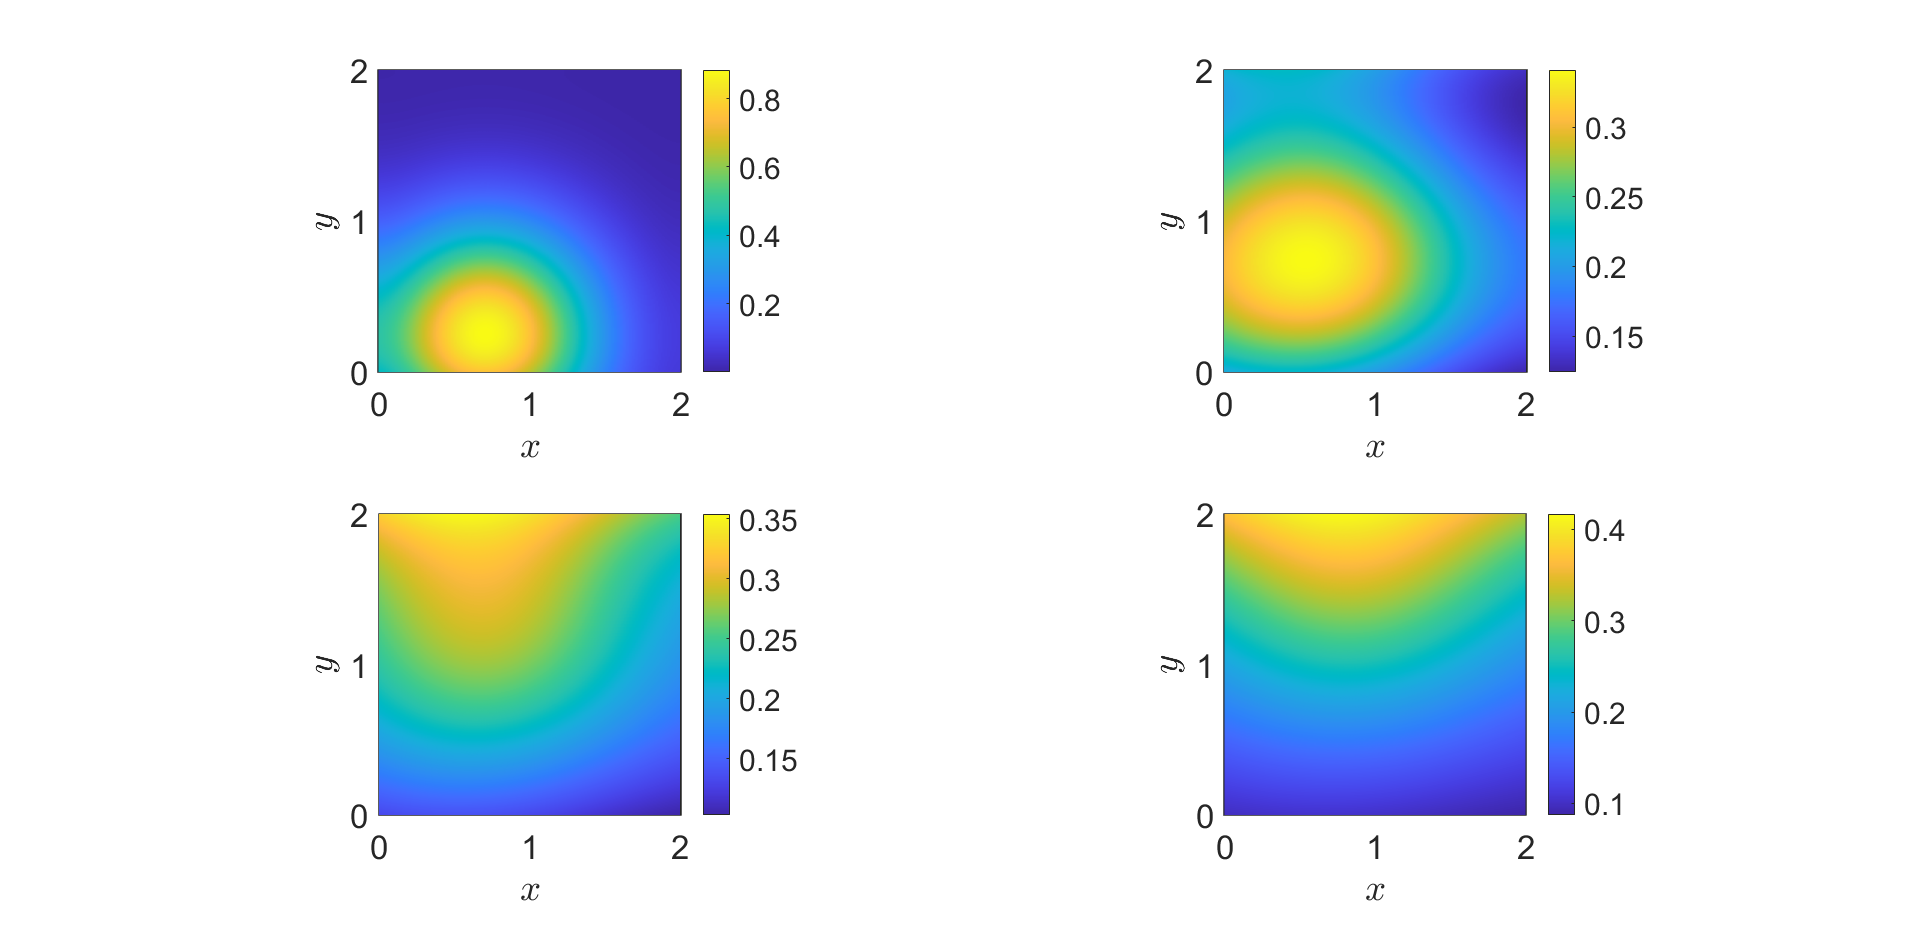
\includegraphics[scale=0.35]{FWBox.png}
	\caption{Forward Example on box discretizations} 
	\label{FFW1}
\end{figure}


We follow the same idea, but now consider the wedge discretizations, see Figure \ref{F4}. We choose the initial condition for $\rho$ to be
\begin{align*}
	\rho_0 = \exp(-2((y_1 - 1.5 )^2 + (y_2 - 4.5)^2)),
\end{align*}
and impose a constant flow of strength $3$ acting from left to right, along the angular direction.
We choose $N = 20$ and $N = 30$. The errors are displayed in Table \ref{Tab4:ErrorsFWWedge} and the result can be seen in Figure \ref{FFW2}. 

\begin{table}
	\caption{Errors (compared to whole wedge (h) ) for different discretization (into two and three shapes) of the wedge}
	\begin{tabular}{ ||c| c| c| c|| }
		\hline
		\hline
		& i & j &k\\ 
		\hline
		Abs. Error, $N =20$& $0.0233 $ & $0.0750 $ & $0.0189 $ \\  
		Rel. Error, $N =20$& $0.0026 $& $0.0068 $ &$0.0013 $ \\
		Abs. Error, $N =30$& $0.0071 $ & $0.0316 $ & $0.0113 $  \\  
		Rel. Error, $N =30$ & $0.0005 $& $0.0019 $ &$ 0.0005$  \\
		\hline
		\hline
	\end{tabular}
	\label{Tab4:ErrorsFWWedge}
\end{table}
\begin{figure}[h]
	\centering
	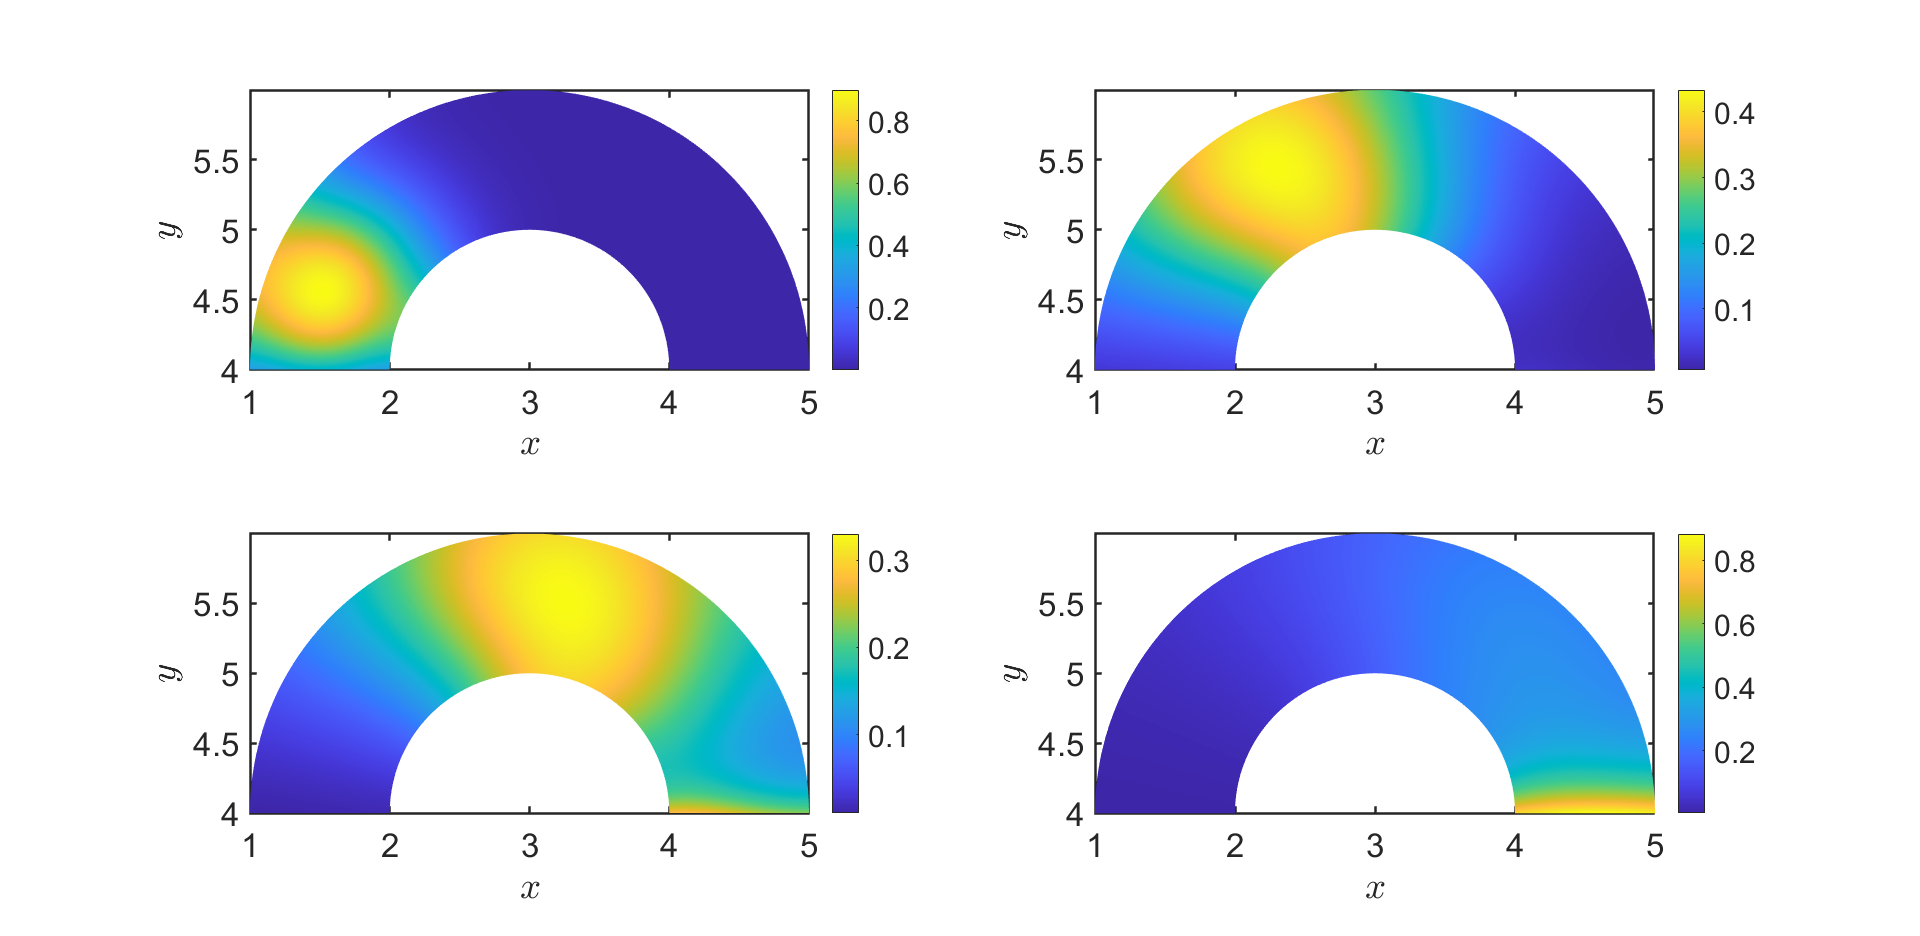
\includegraphics[scale=0.35]{FWWedge.png}
	\caption{Forward Example on wedge discretizations} 
	\label{FFW2}
\end{figure}



Finally, two more complex multishape examples are considered.
The first of these examples is solving an advection diffusion problem on a multishape consisting of two quadrilaterals and two wedges, with constant velocity of strength ten. The initial condition for this problem is:
 \begin{align*}
 	\rho_0 = \exp( -2(y_1 -0.5)^2 - 2 (y_2 + 1)^2).
 \end{align*}
The result, evaluated for $N= 20$ on each shape, can be seen in Figure \ref{F8}.

\begin{figure}[h]
	\centering
	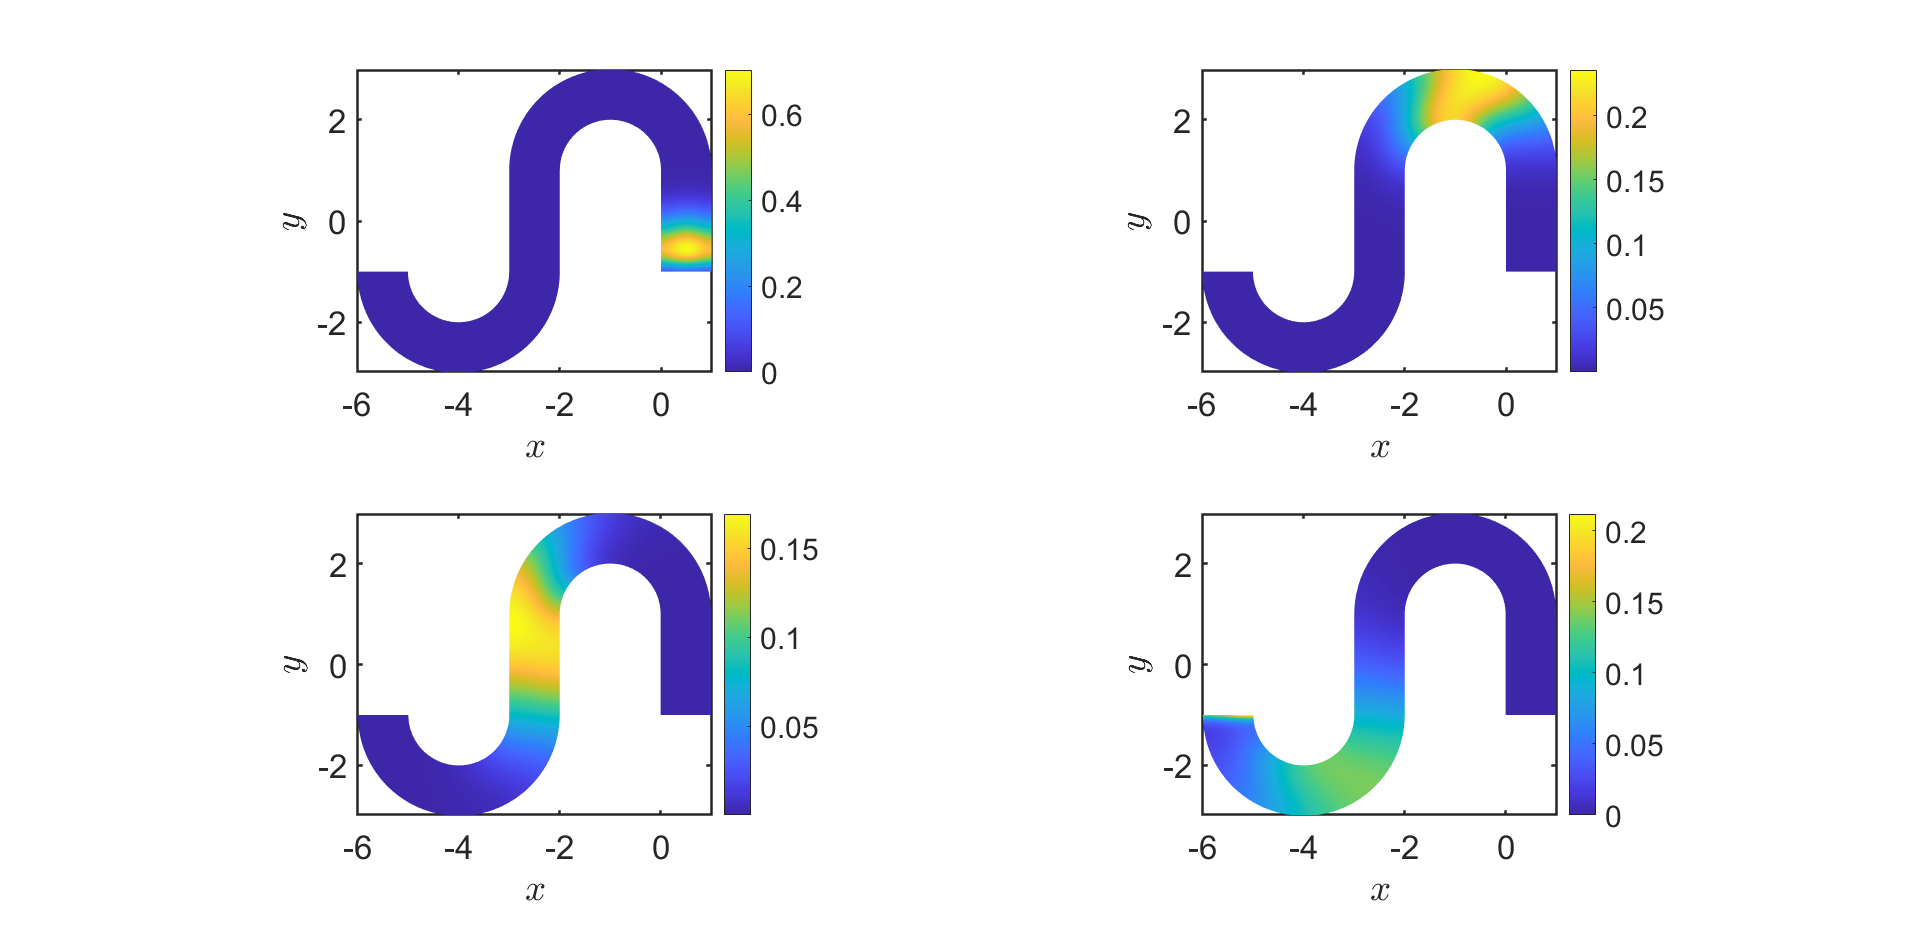
\includegraphics[scale=0.35]{ex1.png}
	\caption{Forward Problem 1, different colour scale for each plot to highlight particle mass location}
	\label{F8}
\end{figure}

In a second example, the velocity is of strength $5$ and the initial condition is:
 \begin{align*}
	\rho_0 = \exp( -2(y_1 -0.5)^2 - 2 (y_2 - 1.5)^2).
\end{align*}
The result, which is computed on a multishape made up of four quadrilaterals into a channel, can be seen in Figure \ref{F9}.

\begin{figure}[h]
	\centering
	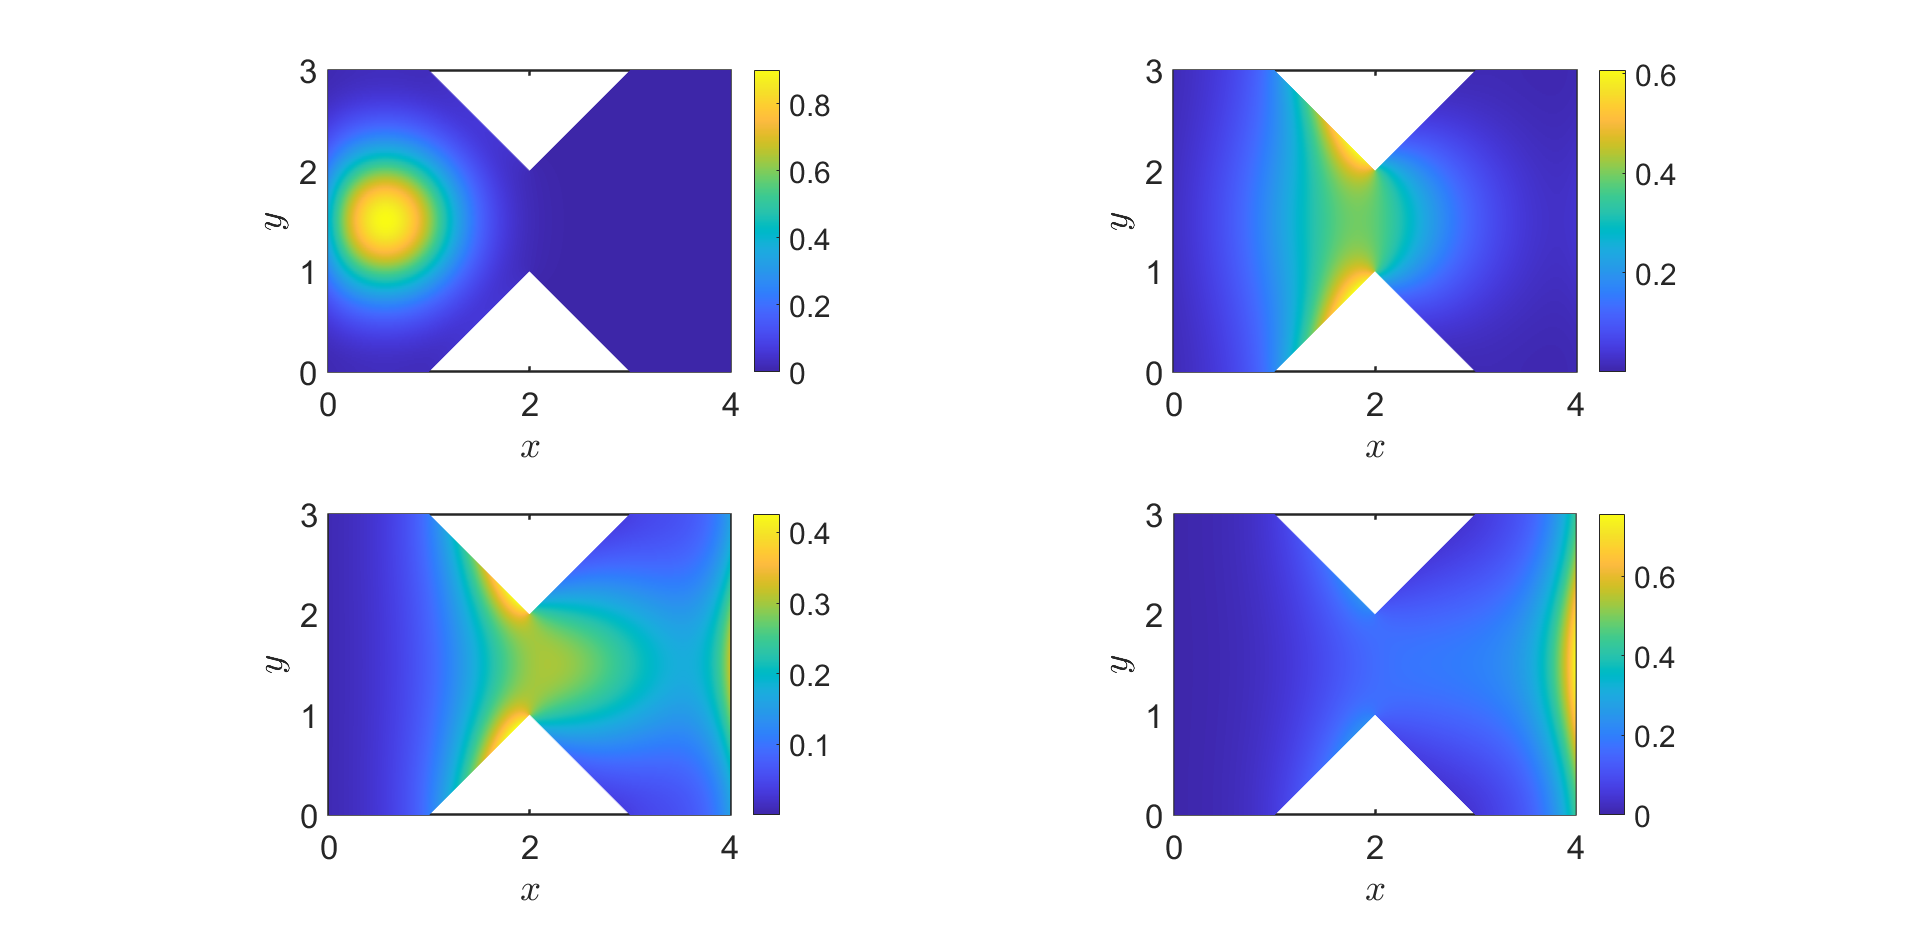
\includegraphics[scale=0.35]{ex2.png}
	\caption{Forward Problem 2, different colour scale for each plot to highlight particle mass location}
	\label{F9}
\end{figure}








\pagebreak	
\bibliography{GeneralBib}
\bibliographystyle{unsrt}
\end{document}